\pagestyle{simple}
\chapter[]{Introdução}

	O multiculturalismo propõe a valorização e convivência harmônica entre diferentes culturas, promovendo o respeito às diversas identidades étnicas, religiosas, linguísticas e sociais dentro de um mesmo espaço. No entanto, mesmo em ambientes onde se busca a inclusão e o respeito à diversidade, como a escola, ainda ocorrem manifestações de violência que comprometem o desenvolvimento saudável dos estudantes. Entre essas manifestações, o bullying físico se destaca como uma das formas mais visíveis e prejudiciais de agressão no contexto escolar. 
	
	A violência representa uma ameaça significativa ao processo educacional, comprometendo a aprendizagem e afetando, a curto e longo prazo, a vida emocional, social e acadêmica da vítima. O termo bullying é utilizado para definir comportamentos agressivos, intencionais e repetitivos, praticados dentro de uma relação desigual de poder, com o objetivo de intimidar, humilhar ou agredir outra pessoa. Essas ações podem ocorrer por meio de agressões físicas, apelidos ofensivos, intimidações, exclusões e zombarias – práticas diretas ou indiretas que causam danos físicos e psicológicos. 
	
	No Brasil, adota-se o termo bullying da literatura internacional, sendo compreendido como um subconjunto de comportamentos violentos e repetitivos. Segundo Fante (2011), para que uma ação seja classificada como bullying, é necessário que ocorra ao menos três vezes ao longo do ano letivo. De forma semelhante, \citeonline{DanOlweus}, um dos principais estudiosos sobre o tema, define que o bullying está presente quando há repetição de atos violentos, de três a cinco vezes por ano, dentro de uma relação desequilibrada de poder entre agressor e vítima. 
	
	As causas da agressividade podem estar relacionadas a diversos fatores, como transtornos comportamentais, influência do meio familiar ou do grupo de convivência, problemas emocionais, entre outros. \citeonline{BeatrizPereira} destaca que o bullying possui três características fundamentais: ausência de provocação por parte da vítima, repetição das agressões e desequilíbrio de força entre os envolvidos. \citeonline{DanOlweus} acrescenta que a escola, infelizmente, tem sido vista cada vez mais como espaço de violência e exclusão, o que exige atenção especial de professores e educadores aos sinais de instabilidade emocional e afetiva dos alunos. 
	
	
	Com base nesse cenário, o presente projeto integrador foi desenvolvido com os alunos do 3º ano do ensino fundamental da Escola Estadual Presidente João Goulart, localizada no extremo sul de São Paulo/SP. Dentro da proposta temática do multiculturalismo, optou-se por abordar especificamente o bullying físico, investigando suas causas, consequências e formas de prevenção em um contexto de diversidade cultural. 
	
	Como recurso pedagógico, será utilizada a literatura infantil, por meio do livro "\textit{E se fosse com você?}", da autora Sandra Saruê. A obra servirá como ponto de partida para atividades de reflexão, promovendo discussões sobre empatia, respeito às diferenças e os impactos do bullying no ambiente escolar.

	\begin{figure}[h]
		\centering
		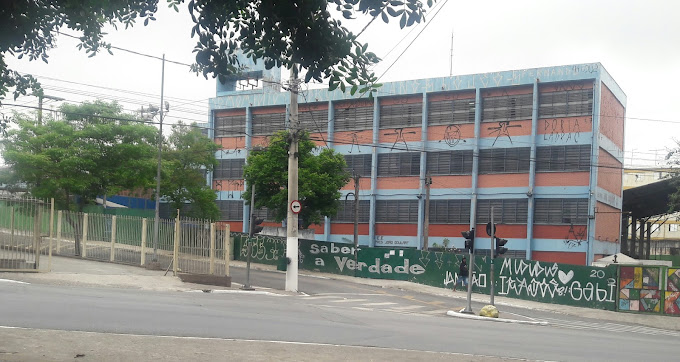
\includegraphics[width=0.75\textwidth]{./imgs_proj/fachada1.jpg}
		\caption{Fachada da E. E. Pres. João Goulart}
		\label{fig:fachada_escola}
	\end{figure}

\chapter{Desenvolvimento}
	O desenvolvimento deste projeto foi pautado em uma pesquisa de campo, com a realização de um estudo de caso junto aos alunos do 3º ano do Ensino Fundamental da Escola Estadual Presidente João Goulart, situada no extremo sul da cidade de São Paulo/SP. 
	
	A partir da observação direta e da interação com a comunidade escolar e o entorno, foram identificadas situações recorrentes de desrespeito entre os alunos, como o uso de apelidos ofensivos, agressões físicas e verbais, exclusão social e comportamentos indisciplinados. Essas evidências revelam um cenário preocupante, que compromete tanto o ambiente escolar quanto o processo de ensino aprendizagem. 
	
	Diante desse contexto, a equipe de pesquisa propôs o desenvolvimento do projeto “Promovendo o respeito às diferenças e combatendo o bullying na escola”, com o objetivo de fomentar uma cultura de paz, por meio de leituras significativas, atividades reflexivas e diálogos sobre a valorização da diversidade e a construção de uma ética multicultural. 
	
	Com isso, nosso grupo acredita que a proposta pedagógica busca não apenas intervir nas relações interpessoais dos alunos, mas também estimular uma reflexão coletiva sobre as práticas escolares e os desafios da convivência em contextos marcados por desigualdades sociais, preconceitos e discriminações. 

	\section{OBJETIVOS}
		\textbf{Objetivo Geral}\\
		Analisar como a valorização do multiculturalismo e das diferenças pode contribuir para a promoção do respeito mútuo e para a redução do bullying no ambiente escolar. 
		
		\textbf{Objetivos Específicos}
		\begin{itemize}[itemsep=0pt, topsep=0pt]
			\item Conhecer diferentes concepções teóricas sobre multiculturalismo e diversidade cultural. 
			\item Levantar situações de bullying relacionadas à intolerância cultural, social ou étnica no contexto escolar. 
			\item Descobrir como os estudantes percebem e vivenciam a diversidade em seu cotidiano escolar. 
			\item Caracterizar o papel da escola na valorização das diferenças culturais e sociais. 
			\item Descrever as principais formas de bullying associadas à discriminação de diferenças (culturais, físicas, religiosas, etc.). 
			\item Determinar os impactos da ausência de práticas multiculturais no convívio escolar. 
			\item Analisar a relação entre multiculturalismo, valorização do outro e a diminuição do bullying. 
			\item Avaliar a eficácia de projetos pedagógicos que promovam o respeito às diferenças. 
			
		\end{itemize}
	
	\section{JUSTIFICATIVA E DELIMITAÇÃO DO PROBLEMA}
	
		Esse projeto justifica-se pela necessidade urgente de enfrentar práticas de bullying físico no ambiente escolar, especialmente em instituições públicas localizadas em regiões mais periféricas, onde as vulnerabilidades sociais são mais visíveis, como é o caso da E.E. Pres. João Goulart, situada no extremo sul da cidade de São Paulo. A ideia é abordar o assunto com os estudantes desenvolvendo habilidades socioemocionais para combater essa prática.
		
		A observação direta realizada com os alunos do 3º ano do ensino fundamental evidenciou comportamentos preocupantes como apelidos ofensivos, agressões físicas, exclusão social e atitudes de desrespeito entre os estudantes. Essas condutas afetam diretamente o ambiente escolar, prejudicando não apenas o rendimento acadêmico, mas também o bem-estar social e emocional dos alunos envolvidos.
		
		Diante desse cenário, a escola vê desafiada a ir além do currículo tradicional, adotando uma abordagem mais humanizada, voltada a formação ética e cidadã. Acreditamos que a escola, enquanto espaço de convivência e construção coletiva, pode e deve promover valores como o respeito, empatia, tolerância e inclusão, especialmente por meio de metodologias que favoreçam o diálogo e a escuta ativa.
		
		A utilização da literatura infantil, representada aqui pelo livro “E Se Fosse Com Você, Uma História de Bullying”, da autora Sandra Saruê, possibilita trabalhar tais valores de forma sensível, acessível e significativa para alunos nessa faixa etária. 
	
	
	\section{FUNDAMENTAÇÃO TEÓRICA}
	
		\subsection{A Escola como Espaço de Convivência e Diversidade}
			
			A escola é um espaço privilegiado de convivência social, onde as diferenças culturais, sociais e emocionais se encontram. Por isso, torna-se fundamental promover ações que incentivem o respeito, a empatia e a valorização da diversidade. Nesse contexto, o multiculturalismo e a prevenção ao bullying devem caminhar juntos, como parte de uma educação voltada para a inclusão e a formação cidadã.
			
			Segundo \citeonline{Candau}, o multiculturalismo na educação busca reconhecer e valorizar as diferentes identidades culturais presentes na escola, promovendo uma pedagogia que respeite a pluralidade e combata toda forma de preconceito e exclusão. A presença da diversidade cultural no ambiente escolar exige dos educadores uma postura atenta às relações entre os alunos, especialmente quando essas relações envolvem comportamentos agressivos ou discriminatórios.
		
		\subsection{O Bullying no Ambiente Escolar}
			A escola, como espaço de formação integral, contribui não apenas para o desenvolvimento de competências cognitivas, mas também para a construção de valores, atitudes e habilidades sociais. No entanto, esse ambiente nem sempre é livre de conflitos, sendo o bullying um dos fenômenos mais recorrentes e prejudiciais ao processo de ensino-aprendizagem e à saúde emocional dos alunos.
			
			Segundo \citeonline{DanOlweus}, o bullying é caracterizado como um comportamento agressivo, intencional e repetitivo, que ocorre em uma relação de desequilíbrio de poder. O bullying físico, especificamente, manifesta-se por meio de empurrões, socos, tapas, chutes e outras formas de violência corporal, frequentemente acompanhadas por ofensas verbais e exclusão social.
			
			\citeonline{IzabelMenezes} destaca que o bullying físico é um dos tipos mais visíveis e, paradoxalmente, um dos mais ignorados, muitas vezes naturalizado como “brincadeiras” ou “coisas de criança”. No entanto, suas consequências são graves e duradouras, afetando o rendimento escolar, a autoestima e a saúde mental das vítimas, além de poder perpetuar ciclos de violência. 
			
		\subsection{Educação Multicultural e respeito às diferenças }
			A valorização da diversidade no ambiente escolar é uma das estratégias mais eficazes no combate ao preconceito e à exclusão. A educação multicultural propõe uma prática pedagógica que reconhece e respeita as identidades culturais, étnicas, religiosas e sociais dos estudantes.
			
			\citeonline{Candau} afirma que a educação multicultural é um caminho para a construção de uma sociedade mais justa, pois promove a convivência ética e solidária desde os primeiros anos escolares. Ao valorizar a pluralidade, a escola contribui para o desenvolvimento da empatia e da consciência crítica dos alunos, ajudando a prevenir atitudes discriminatórias, como o bullying
			
		\subsection{A literatura infantil como estratégia Pedagógica}
			A literatura infantil é uma ferramenta potente para o trabalho com valores humanos e questões sociais, como o respeito à diversidade e a prevenção ao bullying. Segundo \citeonline{Coelho}, a literatura amplia o universo simbólico das crianças, promovendo a identificação com personagens, despertando sentimentos e estimulando a reflexão.
			
			Neste projeto, o livro “\textit{E se fosse você?}”, de Sandra Saruê, foi escolhido por abordar, de maneira sensível e acessível, temas como exclusão, preconceito e empatia. A obra convida os leitores a se colocarem no lugar do outro, o que favorece discussões em sala de aula sobre solidariedade, tolerância e convivência respeitosa. 
			
		\subsection{A Pedagogia do Diálogo e da Escuta}
			Inspirada na pedagogia crítica de Paulo Freire, a proposta do projeto busca promover o diálogo, a escuta ativa e a construção coletiva do conhecimento. Segundo \citeonline{PauloFreire}, o processo educativo deve partir da realidade dos alunos, valorizando suas vivências e suas vozes como ponto de partida para o aprendizado.
			
			No combate ao bullying, essa abordagem é fundamental. Não se trata apenas de aplicar punições isoladas, mas de envolver toda a comunidade escolar em uma reflexão ética e contínua sobre convivência, justiça e responsabilidade social. A pedagogia da escuta propõe ações preventivas, mediadoras e transformadoras, construindo uma verdadeira cultura de paz.
	
	
	\section{METODOLOGIA}
	
		O presente projeto será desenvolvido com a turma do 3º ano do Ensino Fundamental da E.E. Pres. João Goulart, situada no extremo sul de São Paulo/SP, durante o ano letivo vigente.
		
		A metodologia adotada será de caráter qualitativo, baseada em um estudo de caso, que prevê a observação, a interação e a intervenção pedagógica junto aos alunos. As etapas principais serão:
		
		\textbf{Diagnóstico inicial}
		
		Realização de observações em sala de aula e nos momentos de convivência escolar para identificar comportamentos relacionados ao bullying físico e suas possíveis causas, além de entrevistas e conversas informais com professores e alunos para compreender a dinâmica do grupo.
		
		\textbf{Uso da literatura infantil como recurso pedagógico}
		
		Introdução do livro “E se fosse você?”, de Sandra Saruê, para a leitura compartilhada em roda de conversa. A obra será utilizada para estimular a empatia, a reflexão e o diálogo sobre as consequências do bullying e a importância do respeito às diferenças
		
		
		\textbf{Atividades lúdicas e reflexivas}
		
		Proposição de atividades como dramatizações, debates, produções artísticas (desenhos, cartazes, textos) e dinâmicas de grupo, com o objetivo de reforçar os conceitos discutidos durante as rodas de conversa e ampliar a compreensão sobre convivência pacífica.
		
		\textbf{Envolvimento da comunidade escolar}
		
		Organização de encontros com professores, e equipe pedagógica para compartilhar os objetivos do projeto, discutir estratégias de prevenção ao bullying e fortalecer uma rede de apoio à promoção do respeito no ambiente escolar.
		
		\textbf{Registro e análise dos processos}
		
		Documentação das atividades, observações e relatos para acompanhar o desenvolvimento dos alunos e o impacto das ações, possibilitando ajustes na metodologia conforme as necessidades identificadas.
	
	
	\section{RESULTADOS PRELIMINARES: SOLUÇÃO INICIAL} % REMOVER/TROCAR TITULO NA VERSAO FINAL
	
		Diante do diagnóstico realizado junto aos alunos do 3º ano do Ensino Fundamental da Escola Estadual Presidente João Goulart, que evidenciou a presença de comportamentos de bullying físico, o projeto propõe como solução inicial a utilização do livro “E se fosse você?”, de Sandra Saruê, como recurso pedagógico central.
		
		A estratégia consiste em promover rodas de conversa, leituras compartilhadas e atividades lúdicas que incentivem a empatia e o respeito às diferenças, favorecendo a reflexão sobre as consequências das atitudes agressivas e a valorização da diversidade.
		
		Espera-se que, por meio dessas atividades, os alunos desenvolvam maior consciência sobre o impacto do bullying, reconheçam o valor da convivência pacífica e aprimorem suas habilidades sociais para resolver conflitos de maneira não violenta.
		
		Embora ainda não tenha sido implantado, acredita-se que essa abordagem pedagógica, centrada na literatura infantil e no diálogo, será eficaz para reduzir as práticas de bullying físico e promover um ambiente escolar mais acolhedor e seguro.


%\chapter{Resultados}


%\chapter{Considerações Finais}

